\documentclass[professionalfonts]{beamer}
\usepackage{times}
\usepackage{bbm}  % for indicator function
\usepackage{newtxtext,newtxmath}
\usepackage{textpos}
\usepackage{amsmath}
\usepackage{dmtheme}
\usepackage{bibentry}
\usepackage{tcolorbox}
\usepackage{graphicx}
\usepackage{tikz}
\usepackage{amsmath}
\usepackage{verbatim}

\usepackage{lipsum}
\newcommand\blfootnote[1]{		% footnote without a mark
  \begingroup
  \renewcommand\thefootnote{}\footnote{#1}%
  \addtocounter{footnote}{-1}%
  \endgroup
}

%%  TODO:
%%     (1) get a better 'norm' expression rather than $||.||$ 
%%		 (2) remove the citation info from section titles
%%     (3) hyperlinks between pages with relative page numbers
%%     (4) ...


\usetikzlibrary{arrows,shapes}
\usepackage{tikz}

\newcommand*\circled[1]{\tikz[anchor=base, baseline=-.51pt]{	% used for the circled "E" in UESTC in acknowledge frame only 
            \node[shape=circle,fill=org,draw,inner sep=0.08pt,minimum size=.3cm] (char) {#1};}}

\newcommand*\circledchar[1]{\tikz[anchor=base, baseline=-.51pt]{	% char within a circle
            \node[shape=circle,draw,inner sep=0.08pt,minimum size=.3cm] (char) {#1};}}        
\tikzstyle{na} = [baseline=-.5ex]

\tikzstyle{every picture}+=[remember picture]


\beamertemplatenavigationsymbolsempty % remove the navigation symbols
% \beamerdefaultoverlayspecification{<+->}	% pause at every item of itemize

\graphicspath{{image/}} % storage figure in a sub-folder

\usefonttheme{professionalfonts}
\usefonttheme[onlymath]{serif}	% use the article math font for the math equations


% argmax and argmin symbol
\DeclareMathOperator*{\argmax}{arg\,max}
\DeclareMathOperator*{\argmin}{arg\,min}

\title{Matrix Completion and Hawkes Process in Recsys}
\author{((Bai)|(Bo))lin Feng}
\institute[Data Mining Lab, UESTC]{
\includegraphics[height=1.25cm,width=2.5cm]{uestc-dm}\\Data Mining Lab, UESTC}


\date{\today}

\begin{document}

%%%%%%%%%%%%%%%%%%%%%%%%%%%%%%%%%%%%%%%%%  title  %%%%%%%%%%%%%%%%%%%%%%%%%%%%%%%%%%%%%%%%%%%%%%%

\begin{frame}
	\titlepage

	\blfootnote{"Bai" preferred.}
	
\end{frame}

\addtobeamertemplate{frametitle}{
	
	\begin{textblock*}{100mm}(.95\textwidth, 0.1cm)
	
\includegraphics[height=1.4cm,width=1.4cm]{dm-logo}
	\end{textblock*}
}

%%%%%%%%%%%%%%%%%%%%%%%%%%%%%%%%%%%%%%%%%  content  %%%%%%%%%%%%%%%%%%%%%%%%%%%%%%%%%%%%%%%%%%%%%%%
\begin{frame}
	\frametitle{Outline}

	\tableofcontents

	\textbf{Keywords:}\\
{\color{org} 
	{\small \quad recommendation system $\cdot$ matrix completion $\cdot$ Hawkes process}
}
\end{frame}


\begin{frame}{Motivation}
\Large
\textit{"Dear Amazon, I bought a toilet seat because I needed one. Necessity, not desire. I do not collect them. I am not a toilet seat addict."}\footnote[0]{https://twitter.com/GirlFromBlupo/status/982156453396996096}


\end{frame}
%%%%%%%%%%%%%%%%%%%%%%%%%%%%%%%%%%%%%%%%%  content-section 1  %%%%%%%%%%%%%%%%%%%%%%%%%%%%%%%%%%%%%%%%%%%%%%%
%%                            Scalable demand-aware recommendation                                         %%
%%%%%%%%%%%%%%%%%%%%%%%%%%%%%%%%%%%%%%%%%  content-section 1  %%%%%%%%%%%%%%%%%%%%%%%%%%%%%%%%%%%%%%%%%%%%%%%
\section{Matrix Completion and Its Applications}
\subsection{Matrix Completion\cite{Candes2012}\cite{Hsieh2015}}

\begin{frame}{1. Matrix Completion}{(1). Motivation}
Matrix completion is the task of filling in the missing entries of a partially observed matrix.

\begin{equation*}
\left[\begin{array}{llllll}
 {\checkmark} & {?} & {?} & {?} & {\checkmark} & {?} \\
 {?} & {?} & {\checkmark} & {\checkmark} & {?} & {?} \\
 {\checkmark} & {?} & {?} & {\checkmark} & {?} & {?} \\ 
 {?} & {?} & {\checkmark} & {?} & {?} & {\checkmark} \\ 
 {\checkmark} & {?} & {?} & {?} & {?} & {?} \\ 
 {?} & {\checkmark} & {?} & {?} & {\checkmark} & {?} \\ 
 {?} & {?} & {\checkmark} & {\checkmark} & {?} & {?}
 \end{array}\right]
\end{equation*}

\begin{itemize}
\item In general, it is NP-hard.
\item But under additional assumptions, it can be solved efficiently.
\end{itemize}
\end{frame}

\begin{frame}{1. Matrix Completion}{(2). Low-rank Matrix Completion}
Under low-rank restriction (non-convex, still NP-hard):
\begin{equation*}
    \begin{aligned}
    & \underset{X}{\text{min}}
    & & \text{rank}(X) &  \\
    & \text{s.t.} & &  X_{ij} = M_{ij}  & (i,j) \in \Omega
    \end{aligned}
\end{equation*} 

Convex relaxation:\footnote{Candès, Emmanuel J., and Benjamin Recht. \textit{Exact matrix completion via convex optimization}. Foundations of Computational mathematics 9.6 (2009): 717.}
\begin{equation*}
    \begin{aligned}
    & \underset{X}{\text{min}}
    & & ||X||_* &  \\
    & \text{s.t.} & &  X_{ij} = M_{ij}  & (i,j) \in \Omega
    \end{aligned}
\end{equation*} 

Now this can be solved efficiently.
\end{frame}

\subsection{Scalable Demand-Aware Recommendation\cite{Yi2017}}
\begin{frame}{2. Scalable Demand-Aware Recommendation\footnote{Jinfeng Yi, Cho-Jui Hsieh, Kush R. Varshney, etc. \textit{Scalable demand-aware recommendation}. In NIPS, 2017.}}{(1). Motivation}
\begin{itemize}
	\item Item utility $=$ \textit{form utility} $+$ \textit{time utility}.
	\item traditional CF models only considers \textit{form utility} $\rightarrow$ tries to incorporate both utilities.
\end{itemize}
\end{frame}

\begin{frame}{2. Scalable Demand-Aware Recommendation}{(2). PU learning for matrix completion\footnote{Cho-Jui Hsieh, Nagarajan Natarajan, and Inderjit S. Dhillon. \textit{PU learning for matrix completion}. In ICML, 2015.}}
\begin{itemize}
	\item Aims to recover the underlying matrix $M\in \mathbb{R}^{m\times n}$.
	\item $Y$ is a \textbf{clean} 0-1 matrix observed	from $M$ by thresholding process: $Y_{ij} = \mathbbm{1}\{M_{ij}>\tau\}$ and assume that only a subset of positive entries of $Y$ are observed, denoted as $A$. But unfortunately, it is impossible to recover $M$, recover $Y$ instead.
	\item Label-dependent loss:
		\begin{equation*}
		\begin{split}
			\hat{X} &= \argmin\limits_{X: ||X||_*\leq t} \sum_{i,j} \mathit{l}_\alpha(X_{ij}, A_{ij}) \\
				& = \argmin\limits_{X: ||X||_*\leq t} \alpha \sum_{i,j : A_{ij}=1}(X_{ij}-1)^2  + (1-\alpha)\sum_{i,j: A_{ij}=0}X_{ij}^2
		\end{split}
		\end{equation*}
	which can be solved very efficiently by optimization methods.
	\item Recover $Y$ by $\bar{X}_{ij} = \mathbbm{1}\{\hat{X}_{ij}>\tau\}$.
\end{itemize}
\end{frame}

\begin{frame}{2. Scalable Demand-Aware Recommendation}{(3). Loss Functions}
Tensor nuclear norm minimization(TNNM) problem:
\begin{equation*}
\begin{split}
	 \min_{\mathcal{X}\in \mathbb{R}^{m\times n \times l}, \mathbf{d}\in \mathbb{R}^r_+} &
	\eta \sum_{ijk: p_{ijk} = 1}  \max[1 - \overbrace{(\underbrace{x_{ijk}}_{\color{blue} \text{form utility}} - \underbrace{\max(0, d_{c_j}-t_{i c_j k})}_{\color{red} \text{time utility}})}^\text{overall utility}, 0]^2 \\
	& + (1 - \eta) \sum_{ijk: p_{ijk}=0} x_{ijk}^2 + 	\lambda ||\mathcal{X}||^2_*
\end{split}
\end{equation*}

\begin{itemize}
	\item $\mathcal{P} \in  \{0, 1\}^{m\times n \times l}$ denotes the purchase history. 
	\item $\mathcal{X} \in \mathbb{R}^{m \times n \times l }$ denotes the {\color{lbrown} underlying} form utility.
	\item $d \in  \mathbb{R}_+^r$ with $d_i$ denoting the {\color{lbrown} underlying} duration of category $i$.
	\item $\mathcal{T} \in \mathbb{R}^{m \times n \times l}$ where $t_{ic_jk}$ denotes the number of time slots between user $i$'s most recent purchase within item category $c_j$ until time $k$.
	\item A binary utility indicator $\mathcal{Y} \in \{0, 1\}^{m \times n \times l}$ with $$y_{ijk} = \mathbbm{1}[x_{ijk} - \max (0, d_{c_j} - t_{i c_j k}) > \tau].$$
\end{itemize}
\end{frame}

\section{Hawkes Process and Its Applications}
\subsection{Hawkes Process}
%%%%%%%%%%%%%%%%%%%%%%%%%%%%%%%%%%%%%%%%%  content-section 2  %%%%%%%%%%%%%%%%%%%%%%%%%%%%%%%%%%%%%%%%%%%%%%%
%%                                          Hawkes Process                                                 %%
%%%%%%%%%%%%%%%%%%%%%%%%%%%%%%%%%%%%%%%%%  content-section 2  %%%%%%%%%%%%%%%%%%%%%%%%%%%%%%%%%%%%%%%%%%%%%%%

\begin{frame}{3. Hawkes Process\footnote{Patrick J. Laub, Thomas Taimre, Philip K. Pollett. \textit{Hawkes Process}. arXiv:1507.02822.}}
\begin{itemize}
	\item The Hawkes process is a {\color{org} counting process} that models a sequences of 'arrivals' of some type over time and each arrival {\color{org} excites} the process.
	\item Conditional intensity function(CIF) of a counting process $N(t)$ with associated histories $\mathcal{H}(\cdot)$: $$\lambda^*(t) = \lim_{h\rightarrow0} \frac{\mathbb{E}\{N(t+h)-N(t) | \mathcal{H}(t)\}}{h}$$
	\item CIF for Hawkes process: 
		\begin{equation*}
		\lambda^*(t) = 
				\tikz[baseline]{
            \node[fill=org!20, anchor=base] (t1)
            {$\lambda$};
        } + 
				\tikz[baseline]{
            \node[fill=red!20, anchor=base] (t2)
            {$\underset{i:t_i < t}{\sum} \mu(t-t_i)$};
        }
		\end{equation*} 

		\qquad \tikz[baseline]{\node[fill=org!20,anchor=base] (n1) {background intensity};}	\qquad \qquad 
	      \tikz[baseline]{\node[fill=red!20, anchor=base] (n2) {excitation function};}

	  Generally, $\mu(\cdot)$ takes the form of $\mu(t) = \alpha e^{-\beta t}$.
	  
\end{itemize}
\begin{tikzpicture}[overlay]
        \path[->]<1-> (n1) edge (t1);
        \path[->]<1-> (n2) edge (t2);
\end{tikzpicture}
\end{frame}


\begin{frame}{3. Hawkes Process}
	\begin{itemize}
		\item The log-likelihood of the Hawkes model given observations $I$ is:\footnote{Proof can be found in the supplementary material of \cite{Mei2017}}
		\begin{equation*}
			\begin{aligned}
			l &= \left( \sum^k_{i=1} \log P\left( t_i | \mathcal{H}_i\right) \right) + \log P(t_{k+1}>T | \mathcal{H}_I) \\
			&= \sum^k_{i = 1}\log \lambda^*(t_i) - \int^{t_k}_0 \lambda^*(u)\text{d}u
			\end{aligned} 
		\end{equation*}
		
	\end{itemize}
\end{frame}


%%%%%%%%%%%%%%%%%%%%%%%%%%%%%%%%%%%%%%%%%  content-section 2  %%%%%%%%%%%%%%%%%%%%%%%%%%%%%%%%%%%%%%%%%%%%%%%
%%            The Neural Hawkes Process: A Neurally Self-Modulating Multivariate Point Process             %%
%%%%%%%%%%%%%%%%%%%%%%%%%%%%%%%%%%%%%%%%%  content-section 2  %%%%%%%%%%%%%%%%%%%%%%%%%%%%%%%%%%%%%%%%%%%%%%%

\subsection{Neural Hawkes Process\cite{Mei2017}}
\begin{frame}{4. Neural Hawkes Process\footnote{Hongyuan Mei and Jason M Eisner. \textit{The neural hawkes process: A neurally self-modulating multivariate point process}. In NeurIPS, 2017.}}{(1). Motivation}
$$\lambda^*(t) = \lambda + \underset{i:t_i<t}{\sum}\mu(t-t_i)$$
\begin{itemize}
	\item The Hawkes process always assumes that the excitation is \circledchar{1} positive, \circledchar{2} linearly additive over past events, \circledchar{3} exponentially decaying with time.
	\item Neural Hawkes process {\color{org}expands the expressivity} by generalizing it to \circledchar{1} both positive and negative, \circledchar{2}non-linear, \circledchar{3} waving-curve influences.\footnote{\href{https://www.zhihu.com/question/64943934/answer/225960255}{\underline{Author's answer}} at zhihu in Chinese.  } 
		
\end{itemize}
\end{frame}

\begin{frame}{4. Neural Hawkes Process}{(2). A simple generalization}
Original intensity function (with only self-exciting):
$$ \lambda_k(t) = {\color{org} \mu_k} + \sum_{h: t_h < t} {\color{org}\alpha_{k_h, k}} e^{\left(-\delta_{k_h, k}(t-t_h)\right)}, \quad \mu_k{\color{org}\geq 0}, \alpha_{j,k}{\color{org} \geq0}$$

A generalization with self-inhibition:

$$\tilde{\lambda}_k(t) = {\color{org} \mu_k} + \sum_{h: t_h < t} {\color{org} \alpha_{k_h, k}} e^{\left(-\delta_{k_h, k}(t-t_h)\right)},\quad \mu_k{\color{org} \in \mathbb{R}}, \alpha_{j,k}{\color{org} \in \mathbb{R}}$$ 
$$\lambda_k(t) = f_k\left( \tilde{\lambda}_k(t) \right) = s_k \log\left( 1 + \exp\left( \frac{\tilde{\lambda}_k(t)}{s_k} \right) \right)$$

where the "\textit{softplus}" function $f_k(x)$ ensures positive results of the intensity function.
\end{frame}

\begin{frame}{4. Neural Hawkes Process}{(3). The neural generalization}
$$\lambda_k(t) = f_k\left(\boldsymbol{w}_k^\text{T}\boldsymbol{h}(t)\right), \qquad \boldsymbol{h}(t) = \text{cLSTM}(x)$$

\blfootnote{\textbf{cLSTM} stands for \hyperlink{cLSTM}{\textbf{continuous-time LSTM}}.}

\begin{figure}[!ht]
\centering
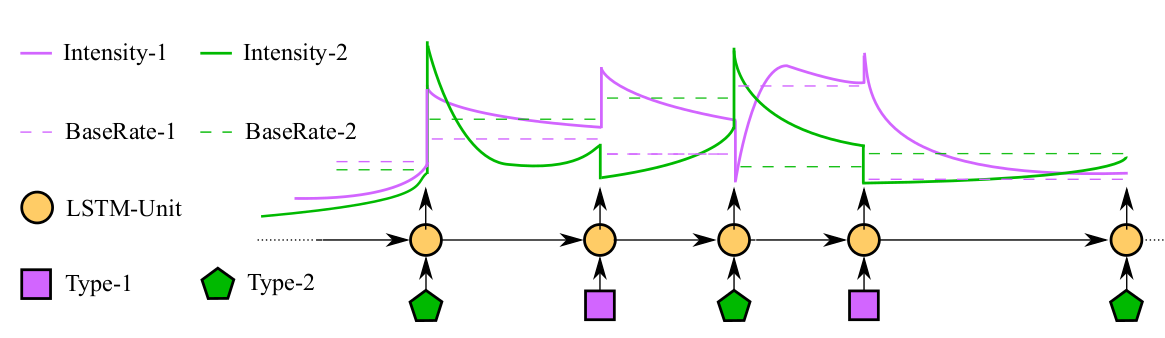
\includegraphics[scale=.35]{Neural_Hawkes_process_demo.png}
\caption[Compact Routing Example]{Drawing an event stream from a neural Hawkes process. Type-1 excites itself but inhibits Type-2. Type-2 excites itself, and excites or inhibits Type-1 according to \#(Type-2) is odd or even.}
\end{figure}
\blfootnote{Image source: \cite{Mei2017}}

\end{frame}

\begin{frame}{4. More About Hawkes Process and Point Process}{(4). References}
Papers:

\begin{itemize}
	\item A Dirichlet Mixture Model of {\color{dbrown} Hawkes Processes} for Event Sequence Clustering, NeurIPS'17\cite{Hongteng2017}
	\item Learning Granger Causality for {\color{dbrown} Hawkes Processes}, ICML'16\cite{Hongteng2016}
	\item Learning {\color{dbrown} Hawkes Processes} from Short Doubly-Censored Event Sequences, ICML'17\cite{Hongteng2017_2}
	\item Learning Conditional Generative Models for Temporal {\color{dbrown} Point Processes}, AAAI'18\cite{Shuai2018}
	\item Wasserstein Learning of Deep Generative {\color{dbrown} Point Process} Models, NeurIPS'17\cite{XiaoFYYYSZ17}
	\item Time is of the Essence: A Joint Hierarchical RNN and {\color{dbrown} Point Process} Model for Time and Item Predictions, WSDM'19\cite{RSA19}
	\item $\cdots$
\end{itemize}

Group: 

\begin{itemize}
	\item Hongyuan Zha @ Georgia Institute of Technology
\end{itemize}
\end{frame}

%%%%%%%%%%%%%%%%%%%%%%%%%%%%%%%%%%%%%%%%%  content-section 3  %%%%%%%%%%%%%%%%%%%%%%%%%%%%%%%%%%%%%%%%%%%%%%%
%%            CTRec: A Long-Short Demands Evolution Model for Continuous-Time Recommendation               %%
%%%%%%%%%%%%%%%%%%%%%%%%%%%%%%%%%%%%%%%%%  content-section 3  %%%%%%%%%%%%%%%%%%%%%%%%%%%%%%%%%%%%%%%%%%%%%%%

\subsection{CTRec\cite{Bai2019}}

\begin{frame}{5. CTRec\footnote{Ting Bai, Lixin Zou, Wayne Xin Zhao, etc. \textit{CTRec: A Long-Short Demands Evolution Model for Continuous-Time Recommendation}. In SIGIR, 2019.}}{(1). Framework: demand-aware Hawkes process}
	\begin{itemize}
		\item Conditional intensity function:
		$$\lambda_{i}(t ; \theta)=f ({\color{org} \underbrace{\boldsymbol{w}_{i}^{\text {item} \top} \cdot \boldsymbol{h}(t)}_{\text{short-term}}} + {\color{mbrown} \underbrace{w_{i}^{\text{attri} \top} \cdot \boldsymbol{\vartheta}(t)}_{\text {long-term }}}+\underbrace{\boldsymbol{w}_{i}^{\text{user} \top} \cdot \boldsymbol{u}}_{\text{basic demands }})$$, where $f(x) = \frac{s}{1 + \exp(\frac{-x}{s})}$.
		\item The parameters here $\boldsymbol{w}_{i}^{\text {item}}$, $\boldsymbol{w}_{i}^{\text {attri}}$, $\boldsymbol{w}_{i}^{\text {user}}$, are learnt by neural Hawkes process.
		\item Then the probability of item $i$ will be purchased at time $t$: $$p_{i}(t ; \theta)=\lambda_{i}(t ; \theta) \exp \left(-\int_{t_{o}}^{t} \lambda_{i}(s ; \theta) d s\right)$$
		\item Expectation next purchase time $\hat{t}_{\text{next}}$ of item $i$ is: $$\hat{t}_{\text{next}} = \int^{+\infty}_{t_o}t\cdot p_i(t;\theta)\text{d}t$$
	\end{itemize}
\end{frame}

\begin{frame}{5. CTRec}{(2). Short-term demands}
	\begin{itemize}
		\item Convolutional representation of item $i_{t_j}$:$$\boldsymbol{v}_{t_{j}}=\operatorname{avg}\left\{\boldsymbol{\imath}_{t_{j}}^{k_{1}}, \ldots, \boldsymbol{\imath}_{t_{j}}^{k_{m}}\right\}$$
		\item Then feed all the item vectors $\boldsymbol{v} = \{\boldsymbol{v}_{t_{1}}, \boldsymbol{v}_{t_{2}},\cdots, \boldsymbol{v}_{t_{n}}\}$ into a time-aware LSTM to capture the short-term demands:
		\begin{equation*}
		\tikz[baseline]{
            \node[fill=org!20,ellipse, anchor=base] (t1)
            {$\boldmath{h}(t)$};
        }
		 = \text{LSTM}(\boldmath{v})
		\end{equation*}
	\end{itemize}

	\begin{tcolorbox}[colback = org!5!white, colframe = org!5!white]
		\begin{equation*}
			\lambda_{i}(t ; \theta)=f ( \underbrace{\boldsymbol{w}_{i}^{\text {item} \top} \cdot  
			% {\color{org}\boldsymbol{h}(t)}
			\tikz[baseline]{
	            \node[fill=org!20,ellipse, anchor=base] (t1)
	            {$\boldmath{h}(t)$};
	        }
			}_{\text{short-term}}  + w_{i}^{\text{attri} \top} \cdot \boldsymbol{\vartheta}(t)+\boldsymbol{w}_{i}^{\text{user} \top} \cdot \boldsymbol{u})
		\end{equation*}
	\end{tcolorbox}

\end{frame}

\begin{frame}{5. CTRec}{(3). Long-term demands}
	\begin{itemize}
		\item Let $\mathcal{D} \in \mathbb{R}^{|U|\times |A| \times |A|}$ be the {\color{org} estimated purchase time distance matrix} of items for all users.
		\item Self-attentive component:$$\alpha_{t, t_{j}}=\boldsymbol{h}\left(t_{j}\right)^{\top} \boldsymbol{i}_{t}-\lambda \log \left(\max \left\{\gamma, d_{a_{t}, a_{t_{j}}}^{u}-\Delta_{a_{t}, a_{t_{j}}}^{u}\right\}\right)$$
		\item Long-term demands: \begin{equation*}
				\tikz[baseline]{
            \node[fill=blue!20,ellipse, anchor=base] (t1)
            {$\boldsymbol{\vartheta}_{t}$};
        }
				=\sum_{j=1}^{n} \frac{\exp \left(\alpha_{t, t_{j}}\right)}{\sum_{q=1}^{n} \exp \left(\alpha_{t, t_{q}}\right)} \boldsymbol{h}\left(t_{j}\right)
		\end{equation*} 

	\end{itemize} 
	\begin{tcolorbox}[colback = blue!5!white, colframe = org!5!white]
	\begin{equation*}
		\lambda_{i}(t ; \theta)=f (\boldsymbol{w}_{i}^{\text {item} \top} \cdot  \boldsymbol{h}(t) +  \underbrace{w_{i}^{\text{attri} \top} \cdot 
		\tikz[baseline]{
            \node[fill=blue!20,ellipse, anchor=base] (t1)
            {$\boldsymbol{\vartheta}_{t}$};
        }
		}_{\text {long-term }}+\boldsymbol{w}_{i}^{\text{user} \top} \cdot \boldsymbol{u})
		\end{equation*}
		\end{tcolorbox} 
\end{frame}


\begin{frame}{5. CTRec}{(4). Loss function}
Maximize the log-likelihood of ovserving items in $I^u_{t_n}$, which can be defined as:\footnote{Hongyuan Mei and Jason M Eisner. \textit{The neural hawkes process: A neurally self-modulating multivariate point process}. In NeurIPS, 2017.}
\begin{equation*}
\begin{aligned} \ell\left(I_{t_{n}}^{u} ; \theta\right) &=\sum_{j=1}^{n} \log \operatorname{Pr}\left(i_{t_{j}} | I_{t_{j}}^{u}, \Delta t_{j}\right) \\ 
&=\underbrace{\sum_{j=1}^{n} \log \lambda_{i_{t_{j}}}\left(t_{j} ; \theta\right)}_{\text {purchase }}-\underbrace{\sum_{i_{\text {neg} \in I}} \int_{t_{1}}^{t_{n}} \lambda_{i_{\text {neg}}}(t) d t}_{\text {non-purchase }} \\ 
&=\sum_{i_{\text {neg}} \in I} \sum_{j=1}^n \left(\frac{1}{|I|} \log \lambda_{i_{t_{j}}}\left(t_{j} ; \theta\right)-\int_{t_{j-1}}^{t_{j}} \lambda_{i_{\text {neg}}}(t) d t\right) \end{aligned}
\end{equation*}
\end{frame}




%%%%%%%%%%%%%%%%%%%%%%%%%%%%%%%%%%%%%%%%%  content-section 4  %%%%%%%%%%%%%%%%%%%%%%%%%%%%%%%%%%%%%%%%%%%%%%%
%%                                    My current research status                                           %%
%%%%%%%%%%%%%%%%%%%%%%%%%%%%%%%%%%%%%%%%%  content-section 4  %%%%%%%%%%%%%%%%%%%%%%%%%%%%%%%%%%%%%%%%%%%%%%%
% \section{My Current Research Status}
% \begin{frame}{6. My Current Research Status}
% \begin{itemize}
% 	\item Nothing
% 	\item Nothing more
% 	\item Literally nothing
% \end{itemize}
% \end{frame}

%%%%%%%%%%%%%%%%%%%%%%%%%%%%%%%%%%%%%%%%%  Q&A  %%%%%%%%%%%%%%%%%%%%%%%%%%%%%%%%%%%%%%%%%%%%%%%
\section{Q\&A}
\begin{frame}[b]
\centering
{\LARGE Q\&A}\\
{\large Thanks!}\\[0.8in]
fengbailin{\color{lblue} n}@gmail.com\\

\includegraphics[height=1.25cm,width=2.5cm]{uestc-dm}\\
Data Mining Lab, U{\color{white} \Large \circled{e}}STC
\end{frame}

%%%%%%%%%%%%%%%%%%%%%%%%%%%%%%%%%%%%%%%%%  content-section 4  %%%%%%%%%%%%%%%%%%%%%%%%%%%%%%%%%%%%%%%%%%%%%%
%%                                           Supplymental                                                 %%
%%%%%%%%%%%%%%%%%%%%%%%%%%%%%%%%%%%%%%%%%  content-section 4  %%%%%%%%%%%%%%%%%%%%%%%%%%%%%%%%%%%%%%%%%%%%%%
\begin{frame}{continuous-time LSTM}
The \hypertarget{cLSTM}{continuous-time LSTM} is defined as follows:
$$\lambda_k(t) = f_k(\boldsymbol{w}_k^\text{T}\boldsymbol{h}(t))$$

$$\boldsymbol{h}(t) = \boldsymbol{o}_i \odot \left( 2\sigma(2\boldsymbol{c}(t)) - 1 \right), \quad \text{for}\; t\in(t_{i-1}, t_i]$$

$$ \boldsymbol{c}(t) \overset{\text{def}}{=} \bar{\boldsymbol{c}}_{i+1} + (\boldsymbol{c}_{i+1}-\bar{\boldsymbol{c}}_{i+1}){\color{org}\exp(-\delta_{i+1}(t-t_i))},\quad \text{for}\;t\in(t_i, t_{i+1}]$$

\blfootnote{\hyperlink{page.13}{Click to go back}}

\end{frame}
%%%%%%%%%%%%%%%%%%%%%%%%%%%%%%%%%%%%%%%%%  bibliography  %%%%%%%%%%%%%%%%%%%%%%%%%%%%%%%%%%%%%%%%%%%%%%%
\begin{frame}[t, allowframebreaks]{Bibliography}
	\bibliographystyle{acm}
	\bibliography{ref}
\end{frame}

\end{document}